\section{Manufacturing company}

\begin{definition}[\textit{Information intensity}]
    Information intensity refers to the amount and complexity of information required in an organization's processes. 
\end{definition}
\noindent Generally, service industries require higher information intensity than manufacturing.
IT Intensity measures how well IT systems meet an organization's information processing needs. 
However, IT intensity can sometimes be greater in manufacturing than in services, depending on automation and digital integration.
\begin{definition}[\textit{Management inclination}]
    Management inclination reflects how much a company's leadership views IT as a strategic asset. 
\end{definition}
\noindent This varies based on factors like digital literacy, organizational culture, and company history.
Historically, manufacturing companies have adopted IT earlier, while service industries experienced a lag of around ten years.

\paragraph*{Drivers}
Several factors determine how IT intensive a company or industry can be:
\begin{enumerate}
    \item \textit{Structure of information processes}: the more structured and rule-based an activity is, the easier it is to automate using IT.
    \item \textit{Data volume}: the sheer amount of information that needs to be processed influences IT requirements.
    \item \textit{Operational frequency}: tasks that are repeated frequently benefit more from IT automation.
    \item \textit{Computational complexity}: simpler processes are easier to digitize and automate efficiently.
\end{enumerate}

\subsection{Manufacturing value chain}
Porter's value chain concept highlights how IT supports various business activities to create competitive advantages.
\begin{figure}[H]
    \centering
    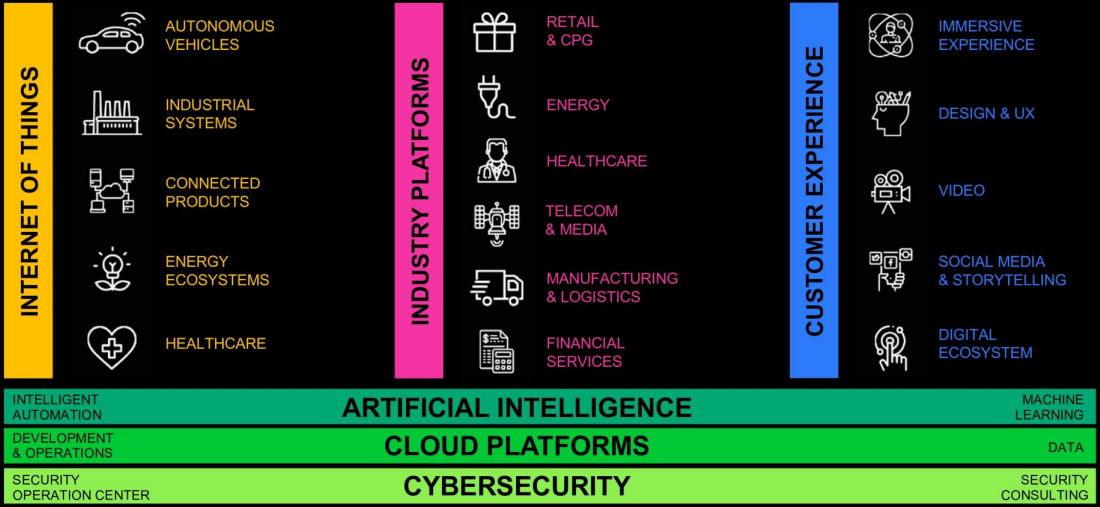
\includegraphics[width=0.75\linewidth]{images/bis2.png}
    \caption{Porter value chain}
\end{figure}

\paragraph*{Activity cycles}
Manufacturing involves continuous, iterative cycles that ensure efficiency and product quality. 
These cycles include:
\begin{enumerate}
    \item \textit{Development cycle}: focuses on designing and industrializing both products and production processes.
    \item \textit{Logistics cycle}: manages customer orders through:
        \begin{itemize}
            \item \textit{Procurement}: acquiring and handling materials, including reception, warehousing, and distribution to production plants.
            \item \textit{Production}: the physical transformation of raw materials into finished goods.
            \item \textit{Sales and distribution}: managing orders, external logistics, and post-sale services such as maintenance and customer support.
        \end{itemize}
\end{enumerate}

\subsection{Inter-functional information processes}
Inter-functional information processes play a key role in managing various aspects of production and operations within a company: 
\begin{enumerate}
    \item \textit{Order management process}: it manages the information regarding orders from order check in to post-sale services.
    \item \textit{Materials management process}: it manages the information regarding materials from outgoing orders towards suppliers to usage within transformation processes.
    \item \textit{Operations management process}: it manages the information regarding operations from materials dispatching to production plants to product delivery.
\end{enumerate}
\noindent These processes are interconnected across different products and divisions within the organization, making the information systems closely tied to the organizational structure. 
All production processes rely on the exchange of information across different functions. 
The use of inter-functional information extends beyond production and operations into planning and control processes. 
It also plays a vital role in administrative tasks.

\subsection{Production}
Companies may produce two types of goods: 
\begin{itemize}
    \item \textit{Standard production}: products have a finite set of predetermined features that can be changed to accommodate customer preferences. 
        In this case, companies produce according to a sales plan, before actual orders are received.
    \item \textit{Custom production}: products are designed according to customer requirements and then produced on demand.
\end{itemize}
\noindent While custom and standard production represent opposite ends of the production spectrum, there is a continuum between the two. 
Custom production is often seen in complex products, while standard production is associated with simpler goods. 
IT supports all production types, although its functionalities vary depending on the degree of customization or standardization in the production process.

\paragraph*{Product structure}
The product structure defines the hierarchical arrangement of components that make up a finished product. 
It ranges from individual components to larger product parts, outlining the relationships and dependencies between them.

\subsection{Information taxonomy}
Operational databases are organized to store various types of information that support the flow of activities within an organization. 
These can be categorized into three primary types: 
\begin{itemize}
    \item \textit{Transaction information}: describes the flow of operational activities, focusing on exchanges between different organizational units and external parties.
        It is the largest in terms of volumes. 
    \item \textit{Operation information}: details the objectives and expected results of operational activities. 
    \item \textit{Catalog information}: basic, static knowledge that exists independently of the flow of production activities. 
        It is quite complex and requires continuous updates and maintenance. 
        This information plays a key role in organizational learning.
\end{itemize}
\noindent Operations planning information is a key link between the operational and the executive portfolios.
Therefore, the level of detail of operational information is a driver of the efficiency of coordination inside an organization.
Operational information has intrinsic value as an organizational asset.
Its usefulness extends beyond internal operations, as it can sometimes be monetized or sold. 

\subsection{Information Technology integration}
Initially, IT functionalities were developed independently for each organizational function, without a comprehensive view of processes. 
The focus was on automating existing activities rather than supporting or re-engineering them to improve performance. 
Each function operated with separate data, and objectives were often misaligned, resulting in inefficiencies.

The traditional approach involved information being created at the start of a cycle and used later. 
However, to truly optimize organizational performance, a more proactive approach is needed. 
This involves using information at the executive level and integrating the various functions within an organization to create a unified view that enhances decision-making and operations.
There are two key approaches to IT integration:
\begin{itemize}
    \item \textit{Horizontal integration}: this refers to the integration of systems along the operating processes of an organization, specifically those that align with Porter's primary processes.
        This is done by the Computer Integrated Manufacturing (CIM), which is a system that supports the integration of manufacturing processes. 
    \item \textit{Vertical integration}: this focuses on connecting the operational portfolio with the executive portfolio. 
        This is done by the Material Requirements Planning (MRP), which ensures materials are available for production at the right time, helping optimize the production process and minimize waste.
\end{itemize}

\paragraph*{Computer Integrated Manufacturing}
CIM integrates various manufacturing processes, with the main objective of achieving an optimal scheduling and production resource management, which results in production efficiency. 
The main functionalities are: activities, workforce, plant, materials and quality management. 

\paragraph*{Materials Requirements Planning}
MRP is a production planning and inventory control system designed to manage manufacturing processes and ensure the availability of materials for production.
It emerged in the 1970s and 1980s with the aim of achieving flexibility and economies of scale through optimal planning. 
This is achieved with concurrent engineering (design and produce in parallel) and inside-out production processes (streamline production processes). 
MRP helps organizations achieve greater effectiveness by allowing them to respond more quickly to market demands while simultaneously benefiting from scale economies. 